\documentclass[10pt]{article}
\usepackage[export]{adjustbox}
\usepackage{amsmath}
\usepackage{array}
\usepackage[makeroom]{cancel}
\usepackage{enumitem}
\usepackage{graphicx}
%Load mhchem using some package options
\usepackage[version=4]{mhchem}
\usepackage{multicol}
\usepackage{siunitx}

\title{
    Problem Set \#10
    \\  \small
    CHEM101A: General College Chemistry
    }
\author{Donald Aingworth}
\date{October 24, 2025}

\newcommand{\E}[1]{\times 10^{#1}}
\newcommand{\hc}{1.9864748\E{-25}\,\unit{\joule\,\meter}}
\newcommand{\U}[1]{\underline{#1}}

\begin{document}
    \DeclareSIUnit{\atm}{atm}
    \DeclareSIUnit{\molarity}{M}
    \DeclareSIUnit{\M}{M}
    \DeclareSIUnit{\torr}{torr}

    \maketitle

    \setcounter{section}{9}

    \pagebreak
    \section{Topic E Problem 23}
        What are the possible values of m$_\ell$ and m$_s$ for a 4f electron?

    \pagebreak
    \section{Topic E Problem 24}
        Explain why it is impossible for an orbital to have n = 3 and $\ell$ = 3. 
        (Hint: think about what these numbers are telling you about nodes.)

    \pagebreak
    \section{Topic E Problem 25}
        The two graphs below show the electron density and radial probability for an atomic orbital.
        (Both graphs show the same orbital.) 
        Use the graphs to answer questions a through e below.
        \begin{center}
            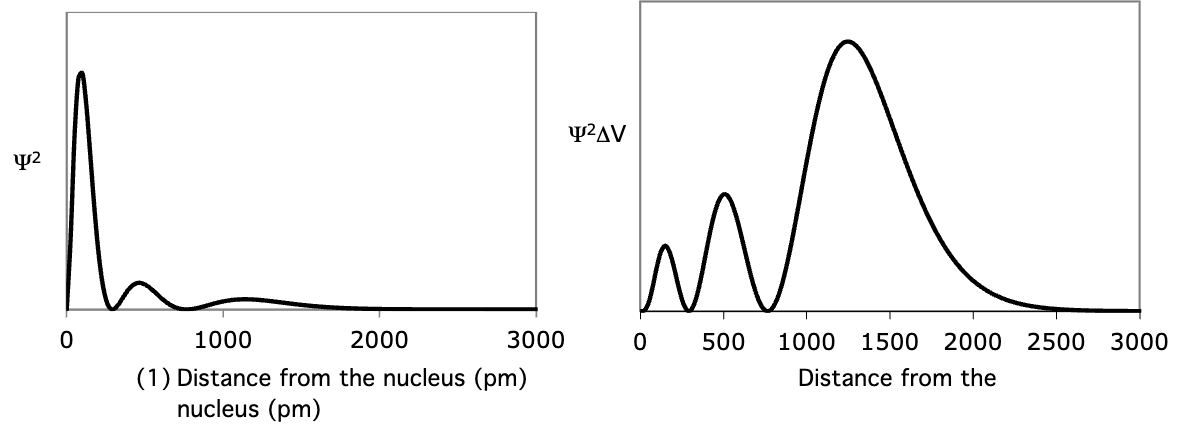
\includegraphics[width=\textwidth]{img-E25.png}
        \end{center}

        \begin{enumerate}[label=\alph*)]
            \item   Which graph is the electron density plot?
            \item   What is the most probable distance between the electron and the nucleus for this orbital? (You will need to estimate it from one of the graphs.)
            \item   How many radial nodes does this orbital have? How can you tell?
            \item   Does this orbital have any angular nodes? How can you tell?
            \item   If n = 4 for this orbital, what orbital is it?
        \end{enumerate}

    \pagebreak
    \section{Topic E Problem 26}
        The radial probability plot below is for a p orbital. 
        What type of p orbital is it (2p, 3p, 4p, etc.)? 
        Explain your reasoning.
        \begin{center}
            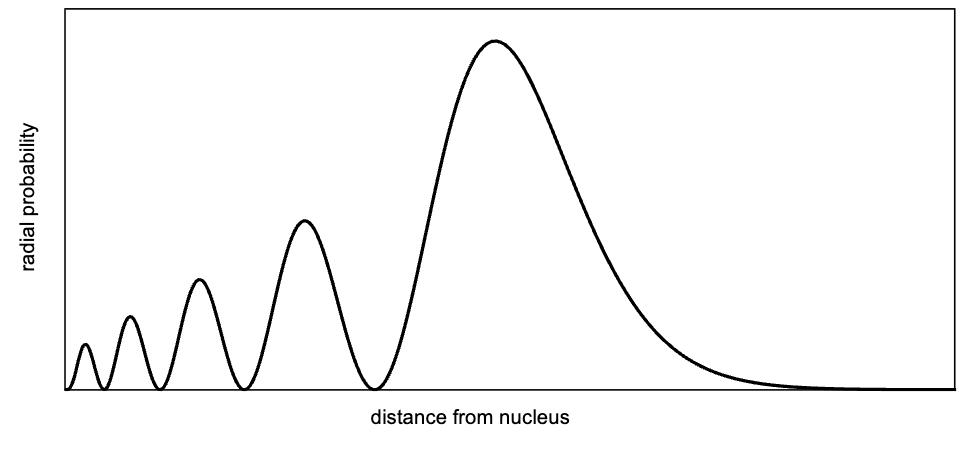
\includegraphics[width=\textwidth]{img-E26.png}
        \end{center}

    \pagebreak
    \section{Topic E Problem 27}
        One of the electron density graphs below is for a 2p orbital and one is for a 3d orbital.
        \begin{enumerate}[label=\alph*)]
            \item   Which one is which? Explain your answer.
            \item   Explain why both of these graphs show just one “hump” (i.e. there is no place where the graph goes to zero).
            \item   Explain why both of these graphs start at the origin.
            \item   Give two examples of orbitals whose electron density plots would not start at the origin, and explain your answer.
        \end{enumerate}
        \begin{center}
            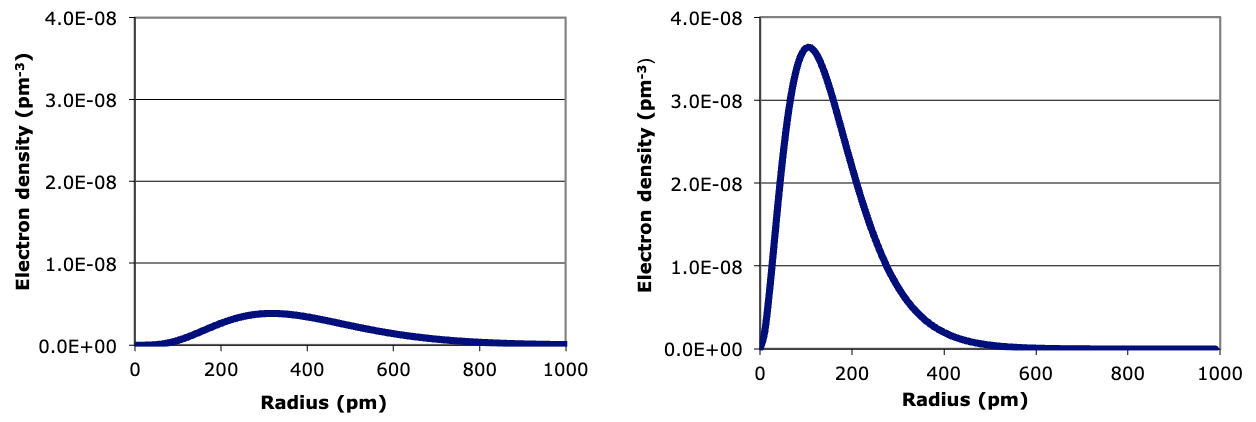
\includegraphics[width=\textwidth]{img-E27.png}
        \end{center}

    \pagebreak
    \section{Topic E Problem 28}
        A partial energy diagram for lithium (Li) is shown below. 
        Answer questions a through d, using the information on this diagram and your understanding of emission spectra. 
        This is a review problem.
        \begin{center}
            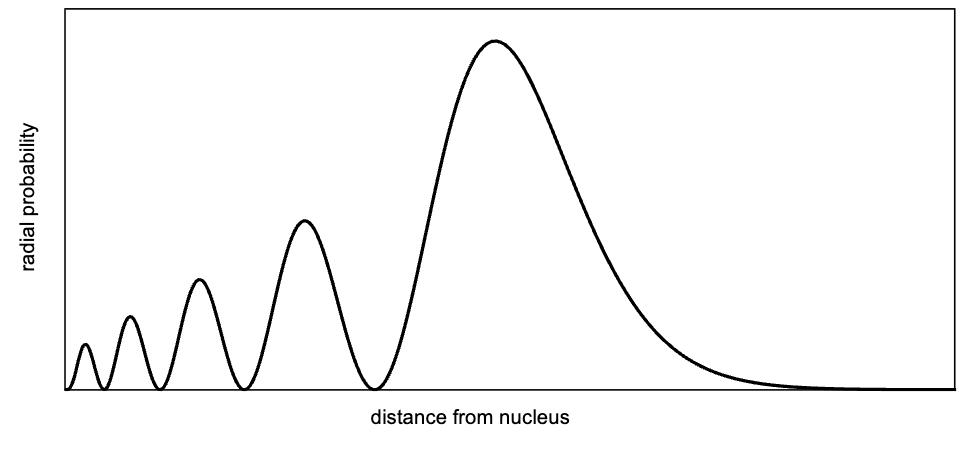
\includegraphics[width=0.5\textwidth]{img-E26.png}
        \end{center}

        \begin{enumerate}
            \item   Calculate $\Delta$E for the 2p $\rightarrow$ 2s transition in lithium, in kJ/mol.
            \item   Calculate the wavelength of light emitted during the 2p $\rightarrow$ 2s transition, in nm.
            \item   When the outer electron undergoes a 5p $\rightarrow$ 2s transition, the atom emits 256nm light. Calculate the energy of the 5p orbital, in kJ/mol.
        \end{enumerate}

    \pagebreak
    \section{Topic E Problem 29}
        Write ground-state electron configurations for the following atoms and ions. 
        You may use inert gas abbreviations (for example, [Ne]3s$^1$ instead of $\rm 1s^2 2s^2 2p^6 3s^1$).
        \begin{multicols}{3}
            \begin{enumerate}
                \item   Rb
                \item   Rb$^+$
                \item   S
                \item   S$^{2-}$
                \item   Cd
                \item   Cd$^{2+}$
                \item   Co
                \item   Co$^{2+}$
                \item   Co$^{3+}$
            \end{enumerate}
        \end{multicols}

    \pagebreak
    \section{Topic E Problem 30}
        \begin{enumerate}[label=\alph*)]
            \item   Which has the higher energy in a hydrogen atom, the 3s orbital or the 3p$_x$ orbital?
            \item   Which has the higher energy in a phosphorus atom, the 3s orbital or the 3px orbital?
            \item   Which has the higher energy in a hydrogen atom, the 4s or the 3dxy orbital?
            \item   Which has the higher energy in a Mn atom, the 4s or the 3dxy orbital?
            \item   Which has the higher energy in a Mn2+ ion, the 4s or the 3dxy orbital?
        \end{enumerate}

    \pagebreak
    \section{Topic E Problem 31}
        Which of the following configurations are ground states, which are excited states, and which are impossible configurations for an uncharged lithium atom?
        \begin{multicols}{3}
            \begin{enumerate}
                \item   1s$^3$
                \item   $\rm 1s^2 1p^1$
                \item   $\rm 1s^2 2s^1$
                \item   $\rm 1s^2 2p^1$
                \item   $\rm 1s^2 87f^1$
            \end{enumerate}
        \end{multicols}


    \pagebreak
    \section{Topic E Problem 32}
        One possible electron configuration for an oxygen atom is [He]$\rm 2s^2 2p^4$. 
        Which of the following orbital energy diagrams represent the ground state, which represent excited states, and which represent impossible arrangements for the 2p electrons in an uncharged oxygen atom?
        \begin{center}
            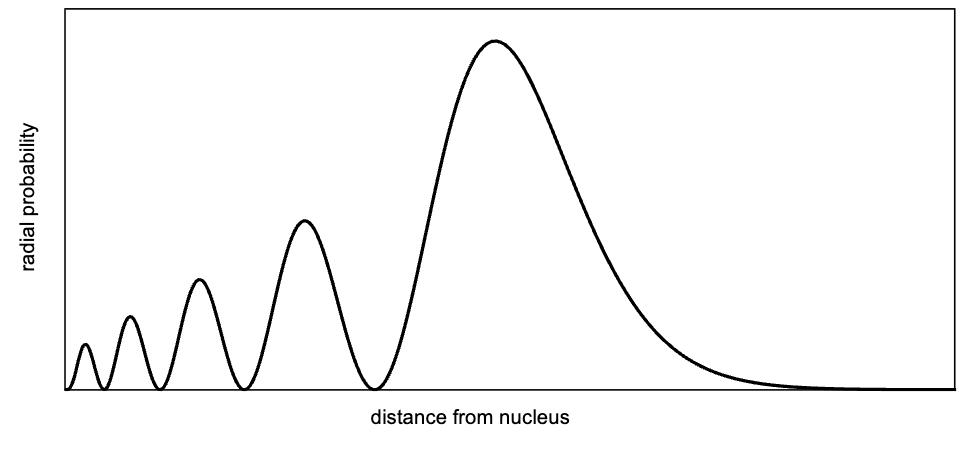
\includegraphics[width=0.75\textwidth]{img-E26.png}
        \end{center}    


    \pagebreak
    \section{Topic E Problem 33}
        Draw orbital energy diagrams for the 3d and 4s orbitals in the ground states of the following atoms. 
        Do not show any other orbitals (but include arrows for the electrons).
        \begin{multicols}{3}
            \begin{enumerate}[label=\alph*)]
                \item   Mn
                \item   Ni
                \item   Mn$^{2+}$
            \end{enumerate}
        \end{multicols}

    \pagebreak
    \section{Topic E Problem 34}
        Which ground-state atoms in period 4 (elements 19 through 36) have…
        \begin{enumerate}[label=\alph*)]
            \item   no unpaired electrons?
            \item   two unpaired electrons?
        \end{enumerate}


    \pagebreak
    \section{Topic E Problem 35}
        Draw an orbital energy diagram for the following configurations.
        \begin{enumerate}
            \item   An atom that has the configuration $\rm 1s^2 2s^2 2p^4$ and is diamagnetic.
            \item   An atom that has the configuration $\rm 1s^2 2s^2 2p^4$ and is paramagnetic.
        \end{enumerate}

    \pagebreak
    \section{Topic E Problem 36}
        Which of the following configurations must be paramagnetic, which could be paramagnetic, and which cannot possibly be paramagnetic (i.e. they must be diamagnetic)?
        \begin{enumerate}[label=\alph*)]
            \item   [Ne]3s
            \item   [Ne]$\rm 3s^2$
            \item   [Ne]$\rm 3s^2 3p$
            \item   [Ne]$\rm 3s^2 3p^2$
        \end{enumerate}


    \pagebreak
    \section{Topic E Problem 37}
        \begin{enumerate}[label=\alph*)]
            \item   How many electrons have n = 4 in a ground-state atom of technetium (Tc)?
            \item   How many electrons have $\ell$ = 1 in a ground-state atom of arsenic (As)?
            \item   How many electrons have m$_\ell$ = 1 in a ground-state atom of krypton (Kr)?
            \item   How many electrons have m$_s$ = $-\frac{1}{2}$ in a ground-state atom of radium (Ra)?
            \item   What is the maximum number of electrons that could have m$_\ell$ = 2 in a ground-state atom of iron?
            \item   What is the minimum number of electrons that could have m$_s$ = $\frac{1}{2}$ in a ground-state atom of oxygen?
        \end{enumerate}


    \pagebreak
    \section{Topic E Problem 38}
        Explain each of the following observations. 
        Explanations such as “Ca is larger than Mg because atoms get larger as you down a column of the periodic table” are not acceptable; you must tell me why this trend occurs.
        \begin{enumerate}[label=\alph*)]
            \item   The atomic radius of Na is larger than the atomic radius of Mg.
            \item   The atomic radius of K is larger than the atomic radius of Na.
            \item   The ionic radius of \ce{S^2-} is larger than the ionic radius of \ce{Cl-}.
            \item   The ionic radius of \ce{Zr^3+} is larger than the ionic radius of \ce{Zr^4+}.
        \end{enumerate}
        

    \pagebreak
    \section{Topic E Problem 39}
        Arrange the elements Al, Ga, Ne, and S in order of increasing ionization energy (i.e. from lowest to highest). 
        You should not need to look up the ionization energies to answer this question.


    \pagebreak
    \section{Topic E Problem 40}
        The list below shows the ionization energies for elements 36 through 40, in kJ/mol:
        \begin{multicols}{3}
            Element 36: 1351\\
            Element 37: 403\\
            Element 38: 549\\
            Element 39: 600\\
            Element 40: 640
        \end{multicols}
        \begin{enumerate}[label=\alph*)]
            \item   Explain why the ionization energies increase as you go from element 37 to element 40.
            \item   Explain why the ionization energy drops dramatically as you go from element 36 to element 37.
            \item   Would you expect the ionization energy of element 35 to be lower than 1351 kJ/mol, or higher than 1351 kJ/mol?
        \end{enumerate}


    \pagebreak
    \section{Topic E Problem 41}
        An element in period 3 (elements 10 through 18) has the following ionization energies.
        Identify the element. 
        Note: IE 1 is the energy required to remove the first electron, IE 2 is the energy required to remove the second electron, etc.
        \begin{multicols}{3}
            IE 1 = 787 kJ/mol\\
            IE 2 = 1577 kJ/mol\\
            IE 3 = 3232 kJ/mol\\
            IE 4 = 4356 kJ/mol\\
            IE 5 = 16,091 kJ/mol\\
            IE 6 = 19,805 kJ/mol
        \end{multicols}


    \pagebreak
    \section{Topic E Problem 42}
        The ionization energy of chlorine is 1251 kJ/mol. 
        Based on this value, which of the following conclusions is reasonable? 
        Select the correct statement, and fill in the blank with the correct orbital name.
        \begin{enumerate}[label=\alph*)]
            \item   The energy of the \_\_\_\_ orbital(s) in chlorine is 1251 kJ/mol.
            \item   The energy of the \_\_\_\_ orbital(s) in chlorine is –1251 kJ/mol.
        \end{enumerate}

    \pagebreak

    \tableofcontents
\end{document}